%% source: 2023-sp-midterm_02
%% tags: [bellman-ford]
\begin{prob}
    Recall that the Bellman-Ford algorithm keeps track of the estimated
    shortest path distance from the source to each node in the graph. These
    estimates are updated, and eventually become correct, provided that the
    graph has no negative cycles.

    Suppose the Bellman-Ford algorithm is run on the graph below using node $s$
    as the source.

    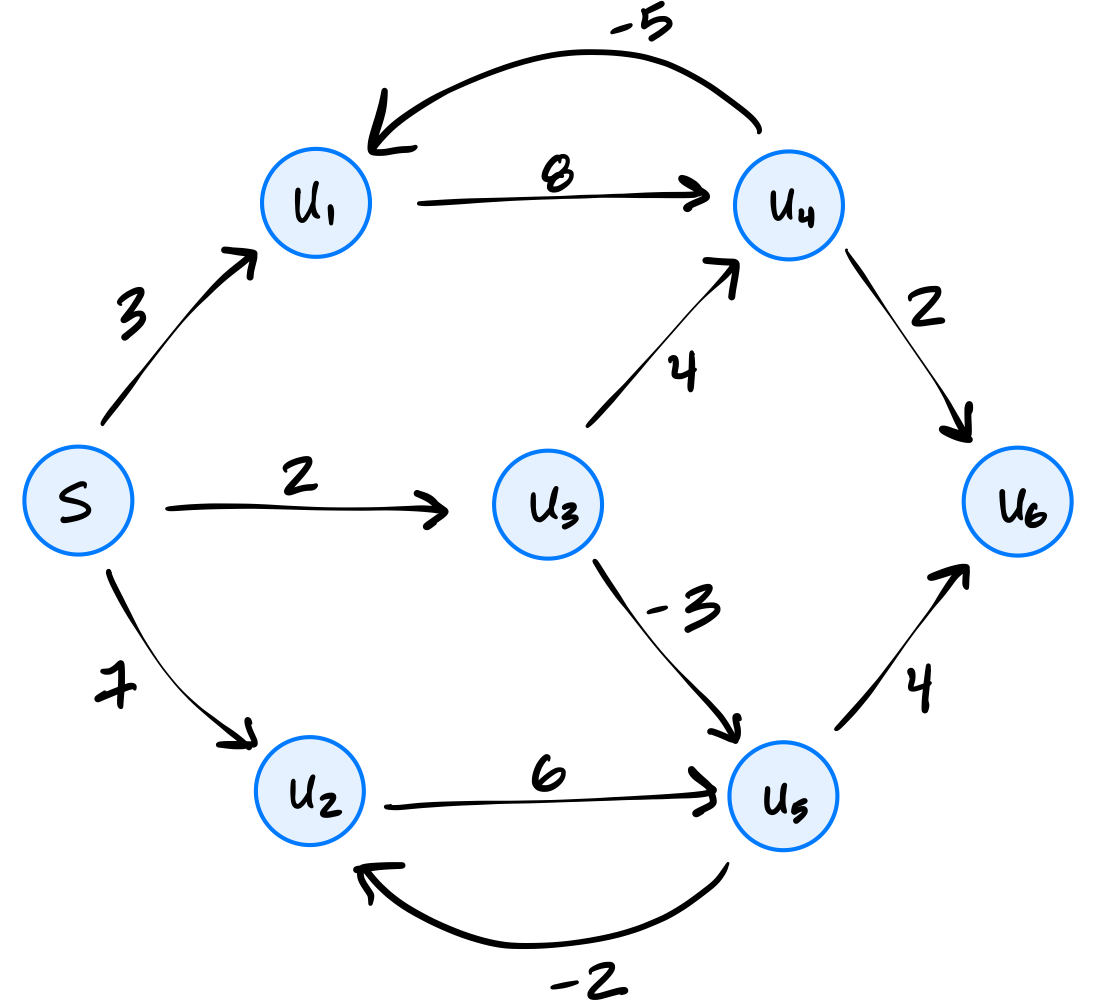
\includegraphics{./graph.png}

    After 2 iterations of the outer loop, which of the nodes listed below are
    guaranteed to have correct estimated shortest path distances (no matter the
    order in which \mintinline{python}{graph.nodes} produces the graph's nodes)? Select all
    that apply.

    \begin{choices}[rectangle]
        \correctchoice $s$
        \choice $u_1$
        \choice $u_2$
        \correctchoice $u_3$
        \correctchoice $u_4$
        \correctchoice $u_5$
        \choice $u_6$
    \end{choices}

    \begin{soln}
        $u_3$, $u_4$, and $u_5$ are guaranteed to have correct estimated shortest path distances after 2 iterations of the outer loop. $s$ is guaranteed to have a correct estimated shortest path distance after 1 iteration of the outer loop.
    \end{soln}


\end{prob}
